%
% loesungsmenge.tex -- Loesungsmenge und Rang
%
% (c) 2009 Prof Dr Andreas Mueller, Hochschule Rapperswil
%
\section{Lösungsmenge und Rang}
\rhead{Lösungsmenge und Rang}
Was passiert, wenn im Gauss-Algorithmus die Anzahl der Gleichungen
nicht mit der Anzahl der Unbekannten übereinstimmt? Oder wenn
plötzlich alle Folgezeilen nur noch Koeffizienten $0$ enthalten,
also auch unter Verwendung der Vertauschungsstrategien kein geeignetes
Pivot-Element mehr zur Verfügung steht? Eine eindeutige Lösung kann
es in diesem Fall natürlich nicht mehr geben.
Die Alternative ``gar keine Lösung'' gegen ``unendlich viele Lösungen''
ist aber noch offen.
Ausserdem ist die Zahl der Gleichungen, nach denen dieses Phänomen
auftritt, eine charakteristische Grösse des betrachteten Gleichungssystems,
der sogenannte Rang.

\subsection{Mehr Unbekannte als Gleichungen}
In diesem Fall kommt das Vorwärtsreduzieren bereits zu einem Ende,
wenn noch gar nicht alle Unbekannten verwendet wurden.
Das Rückwärtseinsetzen kann dann auch nicht alle Spalten ``reinigen'',
so dass rechts einige Spalten stehen bleiben:
\begin{gather}
\definecolor{greenT}{rgb}{0,0.666,0}
\begin{array}{|ccc:cccc|c|}
\hline
1&\dots&0&\color{greenT}*&\dots&\color{greenT}*&&*\\
\vdots&\ddots&\vdots&\vdots&\ddots&\vdots&&\vdots\\
0&\dots&1&\color{greenT}*&\dots&\color{greenT}*&&*\\
\hline
\end{array}
\end{gather}
\index{waehlbar@wählbar}%
Schreibt man dies wieder als System von Gleichungen kann man ablesen,
dass man die Unbekannten $x_{m+1}$ bis $x_n$ gar nicht bestimmen kann.
Diese können frei gewählt werden, und bestimmen dann die Unbekannten
$x_1$ bis $x_m$.
Konkreter: haben wir das Koeffizientenschema
\begin{gather}
\begin{array}{|ccc:cccc|c|}
\hline
1&\dots&0&a_{1,m+1}&\dots&a_{1,n}&&b_1\\
\vdots&\ddots&\vdots&\vdots&\ddots&\vdots&&\vdots\\
0&\dots&1&a_{m,m+1}&\dots&a_{m,n}&&b_m\\
\hline
\end{array}
\end{gather}
gefunden, bedeutet dies, dass die Unbekannten $x_1$ bis $x_m$ bestimmt
sind durch die Gleichungen
{
\definecolor{greenT}{rgb}{0,0.666,0}
\begin{align*}
x_1&=b_1-a_{1,m+1}{\color{greenT}x_{m+1}}-\dots-a_{1n}{\color{greenT}x_n}\\
&\vdots\\
x_m&=b_m-a_{m,m+1}{\color{greenT}x_{m+1}}-\dots-a_{mn}{\color{greenT}x_n}
\end{align*}
}
sobald die Unbekannten $x_{m+1}$ bis $x_n$ frei gewählt werden können.
\subsubsection{Lösungsmenge}
Im vorliegenden Fall hat man eine Lösungsmenge, die durch $n-m$
Parameter beschrieben ist, nämlich durch die frei wählbaren
Variablen $x_{m+1}$ bis $x_n$.
Ein Lösungsvektor hat also die
Form 
\[
\begin{pmatrix}
x_1\\\vdots\\x_m\\x_{m+1}\\\vdots\\x_n
\end{pmatrix}
=
\begin{pmatrix}
b_1-a_{1,m+1}x_{m+1}-\dots-a_{1n}x_n\\
\vdots\\
b_m-a_{m,m+1}x_{m+1}-\dots-a_{mn}x_n\\
x_{m+1}\\
\vdots\\
x_n
\end{pmatrix}
\]
Man spricht von einem $n-m$-dimensionalen Lösungsraum.
Die Lösungsmenge kann also als
\[
\mathbb L
=
\left\{
\,
\left.
\begin{pmatrix}
b_1-a_{1,m+1}x_{m+1}-\dots-a_{1n}x_n\\
\vdots\\
b_m-a_{m,m+1}x_{m+1}-\dots-a_{mn}x_n\\
x_{m+1}\\
\vdots\\
x_n
\end{pmatrix}
\;
\right|
x_{m+1},\dots,x_n\in\mathbb R
\right\}
\]
geschrieben werden.
\subsubsection{Vektorform der Lösungsmenge}
Wir können allerdings auch die Parameter $x_{m+1}$ bis $x_n$ noch
etwas verdeutlichen, indem wir die Lösung als Linearkombination von
Vektoren mit Koeffizienten $x_{m+1}$ bis $x_n$ schreiben:
\[
\begin{pmatrix}
x_1\\\vdots\\x_m\\x_{m+1}\\\vdots\\x_n
\end{pmatrix}
=
\begin{pmatrix}
b_1\\\vdots\\b_m\\0\\\vdots\\0
\end{pmatrix}
+x_{m+1}\begin{pmatrix}
-a_{1,m+1}\\ \vdots\\-a_{m,m+1}\\1\\\vdots\\0
\end{pmatrix}
+\dots+
x_n
\begin{pmatrix}
-a_{1n}\\
\vdots\\
-a_{mn}\\
0\\
\vdots\\
1
\end{pmatrix}
\]
Die Lösungsmenge können wir jetzt etwas kompakter in Vektorform schreiben.
Dazu kürzen wir ab
\[
\tilde b
=
\begin{pmatrix}
b_1\\\vdots\\b_m\\0\\\vdots\\0
\end{pmatrix}
,\qquad
\tilde a_{m+1}=
\begin{pmatrix}
-a_{1,m+1}\\ \vdots\\-a_{m,m+1}\\1\\\vdots\\0
\end{pmatrix}
,\qquad
\tilde a_n
=
\begin{pmatrix}
-a_{1n}\\
\vdots\\
-a_{mn}\\
0\\
\vdots\\
1
\end{pmatrix}
\]
Damit ist die Lösungsmenge
\[
\mathbb L = \{
\tilde b+x_{m+1}\tilde a_{m+1}+\dots+x_n\tilde a_n\;|\;x_{m+1},\dots,x_n\in\mathbb R\}.
\]

\begin{beispiel}
Man bestimme die Lösungsmenge des Gleichungssystems
%   1  -2   3  -0  -4   1
%   3  -1   4  -0   3  -2
%   3  -1   2  -4  -5   4
\[
\begin{linsys}{5}
 x_1&-&2x_2&+&3x_3& &    &-&4x_5&=& 1\phantom{.}\\
3x_1&-& x_2&+&4x_3& &    &+&3x_5&=&-2\phantom{.}\\
3x_1&-& x_2&+&2x_3&-&4x_4&-&5x_5&=& 4.\\
\end{linsys}
\]

\smallskip
{\parindent 0pt Der Gauss-Algorithmus liefert}
\begin{align*}
\begin{tabular}{|>{$}c<{$}>{$}c<{$}>{$}c<{$}>{$}c<{$}>{$}c<{$}|>{$}c<{$}|}
\hline
   1%
\begin{picture}(0,0)
\color{red}\put(-3,4){\circle{12}}
\end{picture}%
& -2&  3&  0& -4&  1\\
   3& -1&  4&  0&  3& -2\\
   3%
\begin{picture}(0,0)
\color{blue}\drawline(-9,-2)(-9,24)(2,24)(2,-2)
\end{picture}%
& -1&  2& -4& -5&  4\\
\hline
\end{tabular}
&
\rightarrow
\begin{tabular}{|>{$}c<{$}>{$}c<{$}>{$}c<{$}>{$}c<{$}>{$}c<{$}|>{$}c<{$}|}
\hline
   1& -2&  3&  0& -4&  1\\
   0&  5%
\begin{picture}(0,0)
\color{red}\put(-3,4){\circle{12}}
\end{picture}%
& -5&  0& 15& -5\\
   0&  5%
\begin{picture}(0,0)
\color{blue}\drawline(-8,-2)(-8,10)(2,10)(2,-2)
\end{picture}%
& -7& -4&  7&  1\\
\hline
\end{tabular}
\\
\rightarrow
\begin{tabular}{|>{$}c<{$}>{$}c<{$}>{$}c<{$}>{$}c<{$}>{$}c<{$}|>{$}c<{$}|}
\hline
   1& -2&  3&  0& -4&  1\\
   0&  1& -1%
\begin{picture}(0,0)
\color{blue}\drawline(-15,24)(-15,-2)(1,-2)(1,24)
\end{picture}%
&  0&  3& -1\\
   0&  0& -2%
\begin{picture}(0,0)
\color{red}\put(-7,4){\circle{15}}
\end{picture}%
& -4& -8&  6\\
\hline
\end{tabular}
&
\rightarrow
\begin{tabular}{|>{$}c<{$}>{$}c<{$}>{$}c<{$}>{$}c<{$}>{$}c<{$}|>{$}c<{$}|}
\hline
   1& -2%
\begin{picture}(0,0)
\color{blue}\drawline(-15,10)(-15,-2)(1,-2)(1,10)
\end{picture}%
&  0& -6&-16& 10\\
   0&  1&  0&  2&  7& -4\\
   0&  0&  1&  2&  4& -3\\
\hline
\end{tabular}
\\
&
\rightarrow
\begin{tabular}{|>{$}c<{$}>{$}c<{$}>{$}c<{$}:>{$}c<{$}>{$}c<{$}|>{$}c<{$}|}
\hline
   1&  0&  0& -2& -2&  2\\
   0&  1&  0&  2&  7& -4\\
   0&  0&  1&  2&  4& -3\\
\hline
\end{tabular}\,.
\end{align*}
Die Variablen $x_4$ und $x_5$ sind frei wählbar, also wird die 
Lösungsmenge:
\[
\mathbb L=
\left\{
\left.
\begin{pmatrix}2\\-4\\-3\\0\\0\end{pmatrix}
+x_4\begin{pmatrix}2\\-2\\-2\\1\\0\end{pmatrix}
+x_5\begin{pmatrix}2\\-7\\-4\\0\\1\end{pmatrix}
\;
\right|
\;
x_4,x_5\in\mathbb R
\right\}.
\]
\end{beispiel}

\subsection{Mehr Gleichungen als Unbekannte}
Sind weniger Unbekannte als Gleichungen gegeben, dann wird das Gauss-Verfahren
das Gleichungssystem bestenfalls in die Form
\[
\begin{array}{|ccc|c|}
\hline
1&\dots&0&*\\
\vdots&\ddots&\vdots&\vdots\\
0&\dots&1&*\\
\hdashline
0&\dots&0&\color{red}*\\
\vdots&\ddots&\vdots&\color{red}\vdots\\
0&\dots&0&\color{red}*\\
\hline
\end{array}
\]
bringen.
Die letzten $m-n$ Zeilen entsprechen Gleichungen, die auf
der linken Seite $0$ stehen haben.
Sie sind nur dann erfüllbar, wenn
auch auf der rechten Seite, an Stelle der Sterne, nur Nullen vorkommen.
Man hat also im Allgemeinen keine Lösung, sondern erst, wenn die Werte
auf der rechten Seite der $m-n$ letzten Gleichungen verschwinden,
also wenn Zusatzbedingungen erfüllt sind.

\subsection{Mischformen}
Es kann auch passieren, dass das Gauss-Verfahren abbricht, bevor alle
Gleichungen aufgebraucht sind, das Schema sieht dann wie folgt aus:
\begin{equation}
\definecolor{greenT}{rgb}{0,0.666,0}
\begin{array}{|ccc:ccc|c|}
\hline
1&\dots&0 &\color{greenT}*&\dots&\color{greenT}*&*\\
\vdots&\ddots&\vdots &\vdots&\ddots&\vdots&\vdots\\
0&\dots&1 &\color{greenT}*&\dots&\color{greenT}*&*\\
\hdashline
0&\dots&0 &0&\dots&0&\color{red}*\\
\vdots&\ddots&\vdots &\vdots&\ddots&\vdots&\color{red}\vdots\\
0&\dots&0 &0&\dots&0&\color{red}*\\
\hline
\end{array}
\label{rangdef}
\end{equation}
In diesem Fall kann man auch durch vertauschen von Zeilen oder Spalten
das Verfahren nach $r$ Gleichungen nicht weiterführen.
Es existiert genau dann eine Lösung, wenn die letzten $m-r$ Gleichungen
mit Nullen auf der linken Seite auch Nullen auf der
rechten Seite haben.

\begin{figure}
\centering
%
% flussdiagrammLoesungsmenge.tex -- Entscheidungsdiagram über Lösbarkeit
%
% (c) 2017 Tabea Méndez, Hochschule Rapperswil
%
\documentclass[tikz]{standalone}
\usepackage{times}
\usepackage{amsmath}
\usepackage{txfonts}
\usepackage[utf8]{inputenc}
\usepackage{graphics}
\usepackage{color}
\usepackage{pifont}
\usetikzlibrary{arrows,shapes.geometric}
\begin{document}

\definecolor{greenT}	{RGB}{0,170,0}

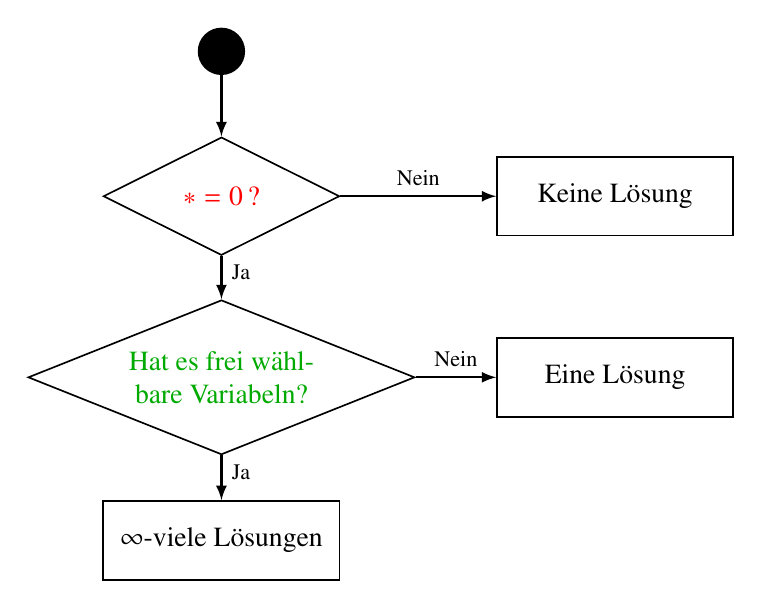
\begin{tikzpicture}[>=latex, scale=1,
    connection/.style={draw=black,thick},
	processStep/.style={rectangle,inner sep=3pt,minimum height=1cm,minimum width=3cm,draw=black,semithick},	
	decision/.style={diamond,inner sep=-1pt,minimum height=1.5cm,minimum width=3cm,draw=black,semithick,aspect=2.5},	
	start/.style={circle,inner sep=0pt,minimum size=16.5pt, draw=black,fill=black,semithick},	
   connection/.style={draw=black,thick,->},
]	

	\def\step{2.3};
	\def\shift{5};



	\node[start](begin) at(0,-0.2*\step){ };
	\node[decision](s0) at(0,-1*\step){\textcolor{red}{$\ast=0\,?$}};
	\node[decision,inner sep=1pt](s1) at(0,-2*\step){\textcolor{greenT}{\parbox{3cm}{\centering Hat es frei wähl-\\ bare Variabeln?}}};

	\node[processStep](s2) at(\shift,-1*\step){Keine Lösung};
	\node[processStep](s3) at(\shift,-2*\step){Eine Lösung};
	\node[processStep](s4) at(0,-2.9*\step){$\infty$-viele Lösungen};


	\draw[connection](begin)--(s0);
	\draw[connection](s0)--node[right,yshift=2pt]{\footnotesize Ja}(s1);
	\draw[connection](s0)--node[above]{\footnotesize Nein}(s2);
	\draw[connection](s1)--node[above]{\footnotesize Nein}(s3);
	\draw[connection](s1)--node[right,yshift=2pt]{\footnotesize Ja}(s4);

\end{tikzpicture}

\end{document}


\caption{Flussdiagramm für die Entscheidung, wieviele Lösungen ein
Gleichungssystem hat, basierend auf dem Schlusstableau
\label{lingl:flussdiagramm}}
\end{figure}

Nehmen wir an, dass auf der rechten Seite der Nullzeilen auch
nur Nullen stehen.
Offensichtlich können nur diejenigen Variablen bestimmt werden,
deren Spalten im Laufe des Verfahrens als Pivot-Spalten aufgetreten sind.
Alle anderen Variablen werden durch die vorhandenen Gleichungen nicht
bestimmt, und sind frei wählbar.

Der gesamte Enscheidungsprozess auf der Basis des
Schlusstableau~\eqref{rangdef} ist im Flussdiagramm
in Abbildung~\ref{lingl:flussdiagramm} zusammengefasst.

\begin{beispiel}
Man finde die Lösungsmenge des Gleichungssystems
\[
\begin{linsys}{4}
x&+&2y&+&3z&=&1\\
x&&&+&z&=&0\\
 &&2y&+&2z&=&1
\end{linsys}
\]
Der Gauss-Algorithmus liefert:
\begin{align*}
\begin{tabular}{|>{$}c<{$}>{$}c<{$}>{$}c<{$}|>{$}c<{$}|}
\hline
1%
\begin{picture}(0,0)
\color{red}\put(-3,4){\circle{12}}
\end{picture}%
&2&3&1\\
1&0&1&0\\
0%
\begin{picture}(0,0)
\color{blue}\drawline(-8,-2)(-8,24)(2,24)(2,-2)
\end{picture}%
&2&2&1\\
\hline
\end{tabular}
&\rightarrow
\begin{tabular}{|>{$}c<{$}>{$}c<{$}>{$}c<{$}|>{$}c<{$}|}
\hline
1&2&3&1\\
0&-2%
\begin{picture}(0,0)
\color{red}\put(-6,4){\circle{15}}
\end{picture}%
&-2&-1\\
0&2%
\begin{picture}(0,0)
\color{blue}\drawline(-8,-2)(-8,10)(2,10)(2,-2)
\end{picture}%
&2&1\\
\hline
\end{tabular}
\\
&\rightarrow
\begin{tabular}{|>{$}c<{$}>{$}c<{$}>{$}c<{$}|>{$}c<{$}|}
\hline
1&2%
\begin{picture}(0,0)
\color{blue}\drawline(-8,9)(-8,-2)(1,-2)(1,9)
\end{picture}%
&3&1\\
0&1&1&\frac12\\
0&0&0&\color{red}0\\
\hline
\end{tabular}
\rightarrow
\begin{tabular}{|>{$}c<{$}>{$}c<{$}:>{$}c<{$}|>{$}c<{$}|}
\hline
1&0&1&0\\
0&1&1&\frac12\\
\hdashline
0&0&0&\color{red}0\\
\hline
\end{tabular}
\end{align*}
Offenbar wird die letzte Gleichung gar nicht benötigt, die
Lösungsmenge kann aus den ersten zwei Gleichungen
abgelesen werden:
\[
\mathbb L=
\left\{
\left.
\begin{pmatrix}
0\\\frac12\\0
\end{pmatrix}
+x_3\begin{pmatrix}
-1\\-1\\1
\end{pmatrix}
\;
\right|\;
x_3\in\mathbb R
\right\}.
\]
\end{beispiel}

\subsection{Definition des Rangs}
\index{Rang}
Offenbar spielt die Zahl $r$, die Anzahl der Einsen im Schema (\ref{rangdef}),
eine wesentliche Rolle, wir nennen diese Zahl den Rang der Matrix.

\begin{definition}
Der Rang einer Matrix $A$ ist die maximale Anzahl linear unabhängiger Zeilen.
\end{definition}
\begin{satz}
Die maximale Anzahl linear unabhängiger Spalten einer Matrix $A$ ist
$\operatorname{Rang}A$.
\end{satz}
Aus dem Rang lässt sich also auch ermitteln, wie viele frei wählbare
Parameter in die Lösungsmenge eingehen.
\begin{satz}
Ist $A$ eine $m\times n$-Matrix mit $r=\operatorname{Rang}A$ 
und $b$ ein $m$-Vektor, dann gibt es $n-r$ Vektoren $\tilde a_1$
bis $\tilde a_{n-r}$ und einen Vektor $\tilde b$ so, dass
\[
\mathbb L
=
\{
\tilde b+x_1\tilde a_1+\dots+x_{n-r}\tilde a_{n+r}\;|\;x_1,\dots,x_{n-r}\in\mathbb R
\}
\]
die Lösungsmenge des Gleichungssystems $Ax=b$ ist.
\end{satz}

\subsection{Reduzierte Zeilenstufenform}
Das allgemeine Schlusstableau der Form (\ref{rangdef}) kann im Allgemeinen nur
erreicht werden, indem nach Bedarf Zeilen- und Spaltenvertauschungen vorgenommen
werden.
Während Zeilenvertauschungen unproblematisch sind, muss man bei
Spaltenvertauschungen sorgfältig darüber Buch führen, zu welcher Variablen
die Spalten gehören.
Dadurch wird der Algorithmus wesentlich komplizierter.
Gewünscht ist eine Variante des Algorithmus, die ohne Zeilenvertauschungen
auskommt, aber immer noch die gleich einfache Interpretation des
Schlusstableaus ermöglicht.

Wir überlegen uns zunächst, wie das Schlusstableau des modifizierten
Algorithmus aussehen müsste.
Das Tableau (\ref{rangdef}) enthält zwei Arten von Spalten:
Spalten mit einer $1$, welche dazu dienen die zugehörte Variable aus der
rechten Seite und eventuell frei wählbaren Variable zu berechnen, und
Spalten mit $*$, die frei wählbare Variablen anzeigen.
Spaltenvertauschungen auf dem Weg zu (\ref{rangdef}) verwenden immer nur Spalten
rechts von der aktuellen Pivot-Spalte, die Spalten links davon sind ja schon
ausgewertet worden.
Tauscht man die Spalten zurück, können zwar Spalten mit $*$ weiter links
landen, aber höchstens so, dass sich links davon eine $1$-Spalte finden
lässt, die die $1$ nicht weiter oben hat als der unterste $*$, das
Tableau sieht also ungefähr so aus:
\begin{center}
\begin{tabular}{| >{$}c<{$} >{$}c<{$} >{$}c<{$} >{$}c<{$} >{$}c<{$} >{$}c<{$} >{$}c<{$} >{$}c<{$} >{$}c<{$} >{$}c<{$} | >{$}c<{$}|}
\hline
1     &0     &*     &0     &0     &*     &0     &\dots &0     &*     &*\\
0     &1     &*     &0     &0     &*     &0     &\dots &0     &*     &*\\
0     &0     &0     &1     &0     &*     &0     &\dots &0     &*     &*\\
0     &0     &0     &0     &1     &*     &0     &\dots &0     &*     &*\\
0     &0     &0     &0     &0     &0     &1     &\dots &0     &*     &*\\
\vdots&\vdots&\vdots&\vdots&\vdots&\vdots&\vdots&\ddots&\vdots&\vdots&\vdots\\
0     &0     &0     &0     &0     &0     &0     &\dots &1     &*     &*\\
\hdashline
0     &0     &0     &0     &0     &0     &0     &\dots &0     &0     &\color{red}*\\
\vdots&\vdots&\vdots&\vdots&\vdots&\vdots&\vdots&\ddots&\vdots&\vdots&\color{red}\vdots\\
0     &0     &0     &0     &0     &0     &0     &\dots &0     &0     &\color{red}*\\
\hline
\end{tabular}
\end{center}
Auch in dieser Form lassen sich die Fragen bezüglich der Anzahl der Lösung
direkt aus dem Tableau ablesen.
Ist einer der roten $\color{red}*$ von Null verschieden, gibt es keine Lösung,
andernfalls gibt es unendlich viele Lösungen, wenn frei wählbare Variablen
in Spalten mit $*$ vorhanden sind.
Die Lösungsmenge lässt sich wieder ablesen, indem man die frei wählbaren
Variablen auf die rechte Seite bringt.

Nachdem nun klar ist, wie ein Schlusstableau ohne Spaltenvertauschungen aussehen
wird, müssen wir den Algorithmus so formulieren, dass wir das Tableau direkt
finden können, ohne Umweg über Vertauschungen und Rückvertauschungen.
Im bisherigen Algorithmus wird eine Spaltenvertauschung unumgänglich, wenn
im nächsten Pivot-Feld und in allen Feldern der Spalte unterhalb des Pivot-Feldes
nur $0$ stehen:
\begin{center}
\begin{tabular}{| >{$}c<{$} >{$}c<{$} >{$}c<{$} >{$}c<{$} >{$}c<{$} | >{$}c<{$} |}
\hline
\qquad\qquad &*     &*     &*     &\qquad\qquad&*     \\
       &\vdots&\vdots&\vdots&      &\vdots\\
       &1     &*     &*     &      &*     \\
       &0     &0\begin{picture}(0,0)
\color{red}\put(-3.5,3){\circle{15}}
\end{picture}&*     &      &*     \\
       &\vdots&\vdots&\vdots&      &\vdots\\
       &0     &0     &*     &      &*     \\
\hline
\end{tabular}
\end{center}
Die zur Pivot-Spalte gehörige Variable kann auf keinen Fall bestimmt werden,
denn dazu wäre ja ein von Null verschiedenes Element an der Pivot-Position
oder darunter notwendig.
Es steht also jetzt schon fest, dass diese Variable frei wählbar ist.
Man kann daher diese Spalte überspringen, und in der nächsten Spalte nach
einem geeigneten Pivot-Element suchen:
\begin{align*}
\begin{tabular}{| >{$}c<{$} >{$}c<{$} >{$}c<{$} >{$}c<{$} >{$}c<{$} | >{$}c<{$} |}
\hline
\qquad\qquad &*     &*     &*     &\qquad\qquad&*     \\
       &\vdots&\vdots&\vdots&      &\vdots\\
       &1     &*     &*     &      &*     \\
       &0     &0     &*
\begin{picture}(0,0)
\color{red}\put(-3.5,3){\circle{15}}
\end{picture}
                            &      &*     \\
       &\vdots&\vdots&\vdots&      &\vdots\\
       &0     &0     &*     &      &*     \\
\hline
\end{tabular}
&\rightarrow
\begin{tabular}{| >{$}c<{$} >{$}c<{$} >{$}c<{$} >{$}c<{$} >{$}c<{$} | >{$}c<{$} |}
\hline
\qquad\qquad&*     &*     &*     &\qquad\qquad&*     \\
            &\vdots&\vdots&\vdots&            &\vdots\\
            &1     &*     &*     &            &*     \\
            &0     &0     &1     &            &*     \\
            &\vdots&\vdots&\vdots&            &\vdots\\
            &0     &0     &0     &            &*     \\
\hline
\end{tabular}
\end{align*}
Die Einsen entstehen jetzt nicht mehr entlang der Diagonalen, sondern
entlang einer Treppe, in der einzelne Stufen auch etwas breiter sein können.
Das Rückwärtseinsetzen funktioniert weiterhin, wobei natürlich nur
Spalten bearbeitet werden können, in denen sich eine Pivot-Position
befindet.

\begin{beispiel}
Man finde die Lösungsmenge des Gleichungssystems
\[
\begin{linsys}{5}
3x&+&6y& &  &+&12v&=& 6\phantom{.}\\
 x&+&2y&+&3z&+&25v&=&17\phantom{.}\\
2x&+&4y&+&3z&+&29v&=&19.
\end{linsys}
\]
In Tableauform vollzieht sich der modifizierte Gauss-Algorithmus jetzt wie
folgt:
\begin{align*}
\begin{tabular}{| >{$}c<{$} >{$}c<{$} >{$}c<{$} >{$}c<{$} | >{$}c<{$} |}
\hline
  3
\begin{picture}(0,0)
\color{red}\put(-3.5,3){\circle{12}}
\end{picture}
   &  6&  0& 12&  6\\
  1&  2&  3& 25& 17\\
  2&  4&  3& 29& 19\\
\hline
\end{tabular}
&\rightarrow
\begin{tabular}{| >{$}c<{$} >{$}c<{$} >{$}c<{$} >{$}c<{$} | >{$}c<{$} |}
\hline
  1&  2&  0&  4&  2\\
  0&  0&  3
\begin{picture}(0,0)
\color{red}\put(-3.5,3){\circle{12}}
\end{picture}
           & 21& 15\\
  0&  0&  3& 21& 15\\
\hline
\end{tabular}
\rightarrow
\begin{tabular}{| >{$}c<{$} >{$}c<{$} >{$}c<{$} >{$}c<{$} | >{$}c<{$} |}
\hline
  1&  2&  0&  4&  2\\
  0&  0&  1&  7&  5\\
  0&  0&  0&  0&  0\\
\hline
\end{tabular}
\end{align*}
Per Zufall ist das Element oberhalb der $1$ in der dritten Spalte auch schon $0$,
es gibt also für das Rückwärtseinsetzen nichts mehr zu tun.

Man kann jetzt die Lösungsmenge ablesen: frei wählbar sind die Variablen 
$y$ und $z$, die Variablen $x$ und $v$ können durch $y$ und $v$ ausgedrückt
werden
\begin{align*}
x&=2-2y-4v\\
z&=5-7v.
\end{align*}
Die Lösungsmenge ist daher
\[
{\mathbb L}
=
\left\{
\left.
\begin{pmatrix}x\\y\\z\\v\end{pmatrix}
=
\begin{pmatrix}2\\0\\5\\0\end{pmatrix}
+y\begin{pmatrix}-2\\1\\0\\0\end{pmatrix}
+v\begin{pmatrix}-4\\0\\-7\\1\end{pmatrix}\;\right|
y,v\in\mathbb R
\right\}.
\]
\end{beispiel}

Das nach diesem modifizierten Algorithmus gefundene Schlusstableau heisst
die {\em reduzierte Zeilenstufenform}, englisch auch {\em reduced row echelon form}.
\index{Zeilenstufenform, reduzierte}
\index{rref}
\index{reduced row echelon form}
Leistungsfähige Taschenrechner und Programme zur Matrizenrechnung stellen
eine üblicherweise \texttt{rref} genannte Funktion zur Verfügung, welche die 
Zeilenstufenform einer beliebigen Matrix berechnen kann.

